\addcontentsline{toc}{chapter}{Appendices}

% The \appendix command resets the chapter counter, and changes the chapter numbering scheme to capital letters.
%\chapter{Appendices}
\appendix
\chapter{Plots and generated output}
\label{Appendix:output}

\section{Mono-Reconstruction}

\subsection{Plots}

\begin{figure}[H]
  \centering
  \begin{subfigure}[b]{0.55\textwidth}
    \centering
    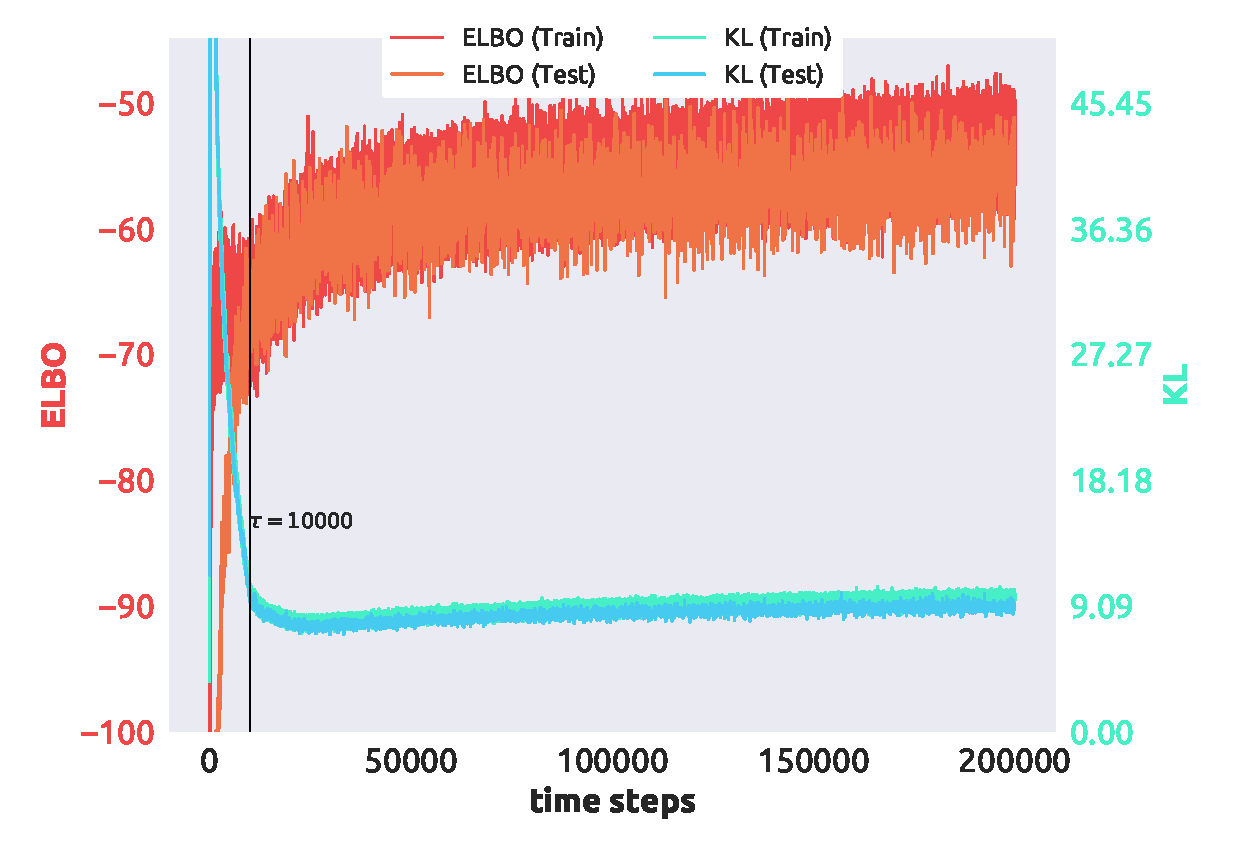
\includegraphics[width=1.0\textwidth]{mlp_reconstruction}
    \caption{Plot for $\mathcal{M}_{M1}$}
    \label{fig:recon_MLP}
  \end{subfigure}
  \begin{subfigure}[b]{0.55\textwidth}
    \centering
    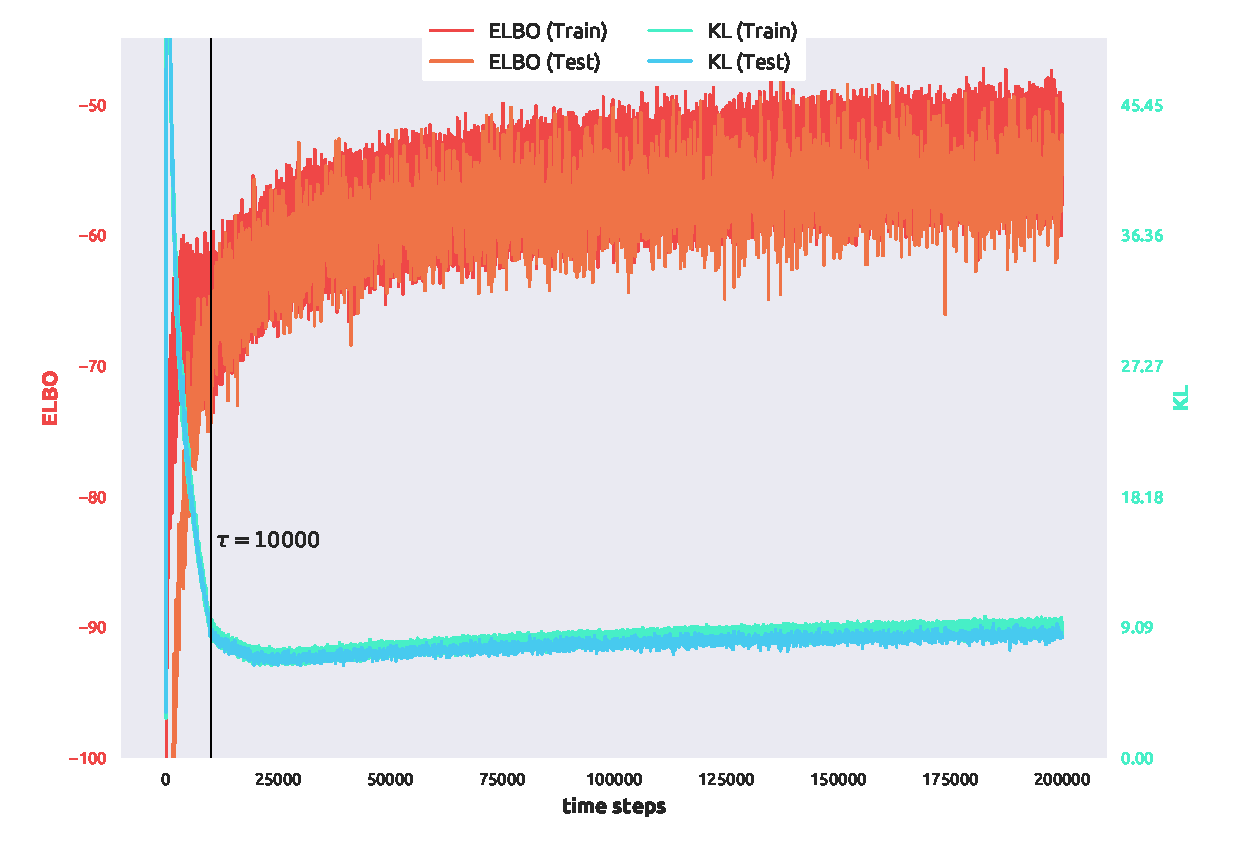
\includegraphics[width=1.0\textwidth]{rnn_reconstruction}
    \caption{Plot for $\mathcal{M}_{M2}$}
    \label{fig:recon_RNN}
  \end{subfigure}
  \begin{subfigure}[b]{0.55\textwidth}
    \centering
    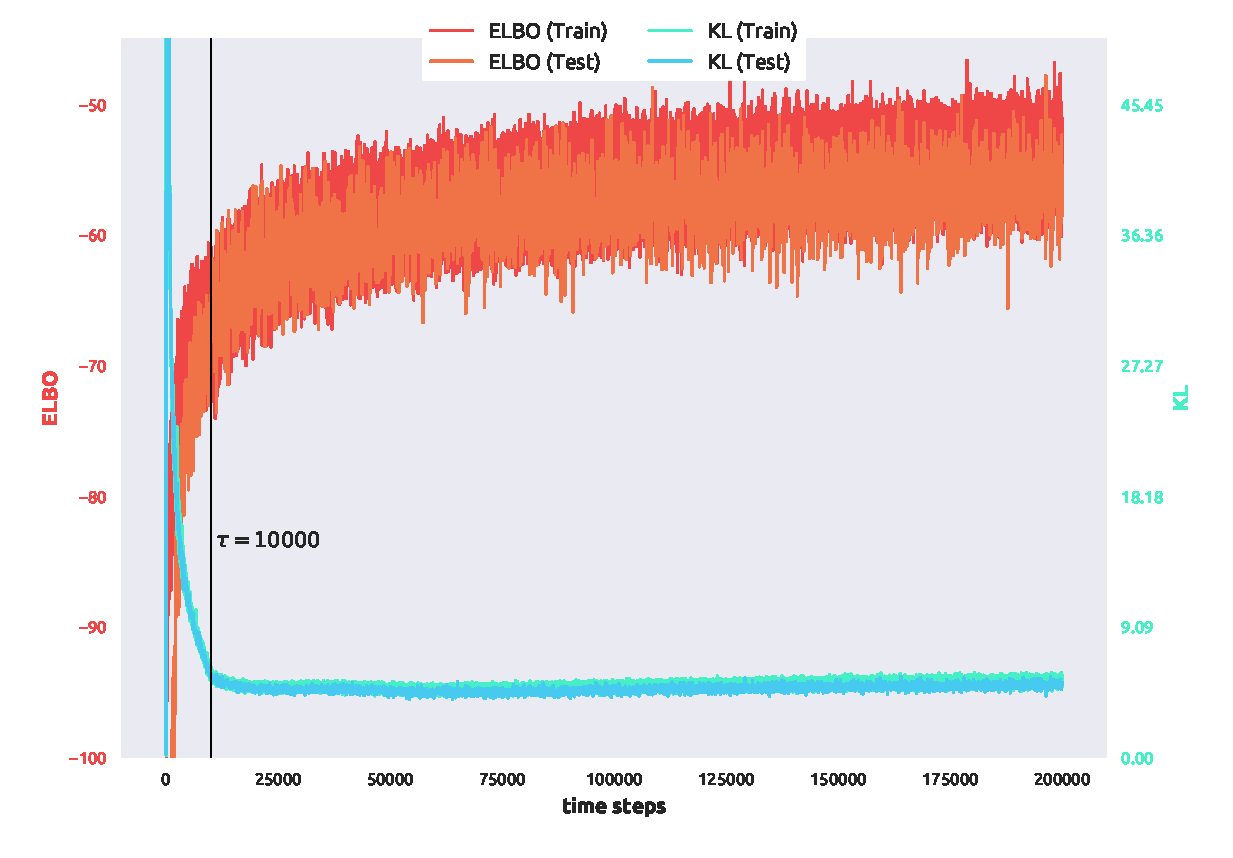
\includegraphics[width=1.0\textwidth]{wavenet_reconstruction}
    \caption{Plot for $\mathcal{M}_{M3}$}
    \label{fig:recon_WaveNet}
  \end{subfigure}
  \caption{Plots of the SGVB estimate of ELBO (Labelled ELBO in plots)
      together with the KL divergence $\KL{q_{\bm{\varphi}}(\bm{z} |
        \bm{x})}{p_{\bm{\theta}}(\bm{z})}$ for the different models for mono-reconstruction. The
      vertical line specifies the end of the KL-annealing.}
\end{figure}

\subsection{Generated Sentences}

\begin{center}
  \begin{tabular}{|c|} 
    \hline
    Sampled sentences from prior (English)\\ [0.5ex] 
    \hline\hline
    Sentences 1\\ 
    \hline
    Sentences 2\\
    \hline
    Sentences 3\\
    \hline
    Sentences 4\\
    \hline
    Sentences 5\\
    \hline
  \end{tabular}
\end{center}

\section{Twin-Reconstruction}

\subsection{Plots}

\begin{figure}[H]
  \centering
  \begin{subfigure}[b]{0.5\textwidth}
    \centering
    \includegraphics[width=1.0\textwidth]{full_fig_mlp_wavenet_translation_fr_en_20-08-17_18:16}
    \caption{Plot for $\mathcal{M}_{T1}$}
    \label{fig:translate_M1}
  \end{subfigure}%
  \begin{subfigure}[b]{0.5\textwidth}
    \centering
    \includegraphics[width=1.0\textwidth]{full_fig_mlp_wavenet_translation_fr_en_22-08-17_11_21}
    \caption{Plot for $\mathcal{M}_{T2}$}
    \label{fig:translate_M2}
  \end{subfigure}
  \begin{subfigure}[b]{0.5\textwidth}
    \centering
    \includegraphics[width=1.0\textwidth]{full_fig_mlp_wavenet_translation_fr_en_28-08-17_20_22}
    \caption{Plot for $\mathcal{M}_{T3}$}
    \label{fig:translate_M3}
  \end{subfigure}%
  \begin{subfigure}[b]{0.5\textwidth}
    \centering
    \includegraphics[width=1.0\textwidth]{full_fig_mlp_wavenet_translation_fr_en_big_dataset_29-08-17_10:36}
    \caption{Plot for $\mathcal{M}_{T4}$}
    \label{fig:translate_M4}
  \end{subfigure}
  \caption{Plots of the SGVB estimate of ELBO (Labelled ELBO in plots)
      together with the KL divergence $\KL{q_{\bm{\varphi}}(\bm{z} |
        \bm{x})}{p_{\bm{\theta}}(\bm{z})}$ for the different models for twin-reconstruction. The
      vertical line specifies the end of the KL-annealing.}
\end{figure}

\subsection{Generated Sentences}

We let (T) stand for the true sentence, and (G) for the generated sentence.

\subsubsection{Model $\mathcal{M}_{M1}$}

\textbf{English}

\begin{center}
  \begin{tabular}{|L{14cm}|} 
    \hline
    Sampled sentences from prior\\ [0.5ex] 
    \hline\hline
    in my view the european union has been said .\\
    \hline
    now we are all UNK ! \\
    \hline
    as far ' s and UNK to being UNK to UNK UNK , to the UNK UNK .\\
    \hline
  \end{tabular}
\end{center}

\begin{center}
  \begin{tabular}{|L{14cm}|} 
    \hline
    Sampled sentences from posterior\\ [0.5ex] 
    \hline\hline
    (T) i find it sad that there are meps who are trying to weaken the commission ' s proposal .\\
    (G) i find it is that the commission , however , the commission is not in the commission .\\
    \hline
    (T) mr president , commissioner , ladies and gentlemen , what is this debate actually about ?\\
    (G) mr president , commissioner , ladies and gentlemen , what is going to do about ?\\
    \hline
    (T) mrs <UNK> was the rapporteur at the time .\\
    (G) mrs <UNK> has to be of no to <UNK> .\\
    \hline
  \end{tabular}
\end{center}

\textbf{French}

\begin{center}
  \begin{tabular}{|L{14cm}|} 
    \hline
    Sampled sentences from prior\\ [0.5ex] 
    \hline\hline
    madame la présidente , ce problème n'est pas tout une intervention des femmes .\\
    \hline
    pouviez , notre groupe aussi pour un communication pour cette approche .\\
    \hline
    lançons , <UNK> a la parole de la commission .\\
    \hline
  \end{tabular}
\end{center}

\begin{center}
  \begin{tabular}{|L{14cm}|} 
    \hline
    Sampled sentences from posterior\\ [0.5ex] 
    \hline\hline
    (T) il est regrettable , selon moi , que certains députés essayent d'affaiblir l'initiative de la commission .\\
    (G) je suis néanmoins qu'il est que la commission que l'on est une proposition pas de la commission .\\
    \hline
    (T) monsieur le président , madame la commissaire , chers collègues , de quoi traite vraiment ce débat ?\\
    (G) monsieur le président , madame la présidente , monsieur le commissaire , dont nous avons ce débat ?\\
    \hline
    (T) à l’époque , c’est mme <UNK> qui était rapporteur .\\
    (G) à occupé de <UNK> , cela était de <UNK> .\\
    \hline
  \end{tabular}
\end{center}

\subsubsection{Model $\mathcal{M}_{M2}$}

\textbf{English}

\begin{center}
  \begin{tabular}{|L{14cm}|} 
    \hline
    Sampled sentences from prior\\
    \hline\hline
    mr president , i see on this report , in the vote .\\
    \hline
    i would like to thank wreckage to hope to be for the european union to be made .\\
    \hline
    you must be able to make for one of one .\\
    \hline
  \end{tabular}
\end{center}

\begin{center}
  \begin{tabular}{|L{14cm}|} 
    \hline
    Sampled sentences from posterior\\ [0.5ex] 
    \hline\hline
    (T) there is a real guerrilla war in progress .\\
    (G) there is a great is the union is .\\
    \hline
    (T) however , later on , while i was asleep , i dreamt of mrs roth-behrendt .\\
    (G) however , as of course , i have , i welcome , i have about .\\
    \hline
    (T) mr president , there is essentially nothing surprising about the situation today .\\
    (G) mr president , there is no longer in the european parliament .\\
    \hline
  \end{tabular}
\end{center}

\textbf{French}

\begin{center}
  \begin{tabular}{|L{14cm}|}
    \hline
    Sampled sentences from prior\\
    \hline\hline
    je tiens à présent à la commission à la commission .\\
    \hline
    nous UNK donc cette décision au conseil .\\
    \hline
    par conséquent ce sont les citoyens .\\
    \hline
  \end{tabular}
\end{center}

\begin{center}
  \begin{tabular}{|L{14cm}|} 
    \hline
    Sampled sentences from posterior\\ [0.5ex] 
    \hline\hline
    (T) une guérilla énorme est en cours .\\
    (G) la russie est en effet est .\\
    \hline
    (T) puis , je me suis quand même UNK , et j'ai rêvé de mme roth-behrendt .\\
    (G) et je tigre , je me UNK , je me UNK , et je me UNK .\\
    \hline
    (T) monsieur le président , la situation d'aujourd'hui n'a au fond rien d'étonnant .\\
    (G) monsieur le président , la situation n'est pas la situation sont la situation .\\
    \hline
  \end{tabular}
\end{center}

\subsubsection{Model $\mathcal{M}_{M3}$}

\textbf{English}

\begin{center}
  \begin{tabular}{|L{14cm}|} 
    \hline
    Sampled sentences from prior\\
    \hline\hline
    to those member states , for proposal for UNK would not support the most people .\\
    \hline
    we would like to make a new measures that of this point .\\
    \hline
    that is something we are now today .\\
    \hline
  \end{tabular}
\end{center}

\begin{center}
  \begin{tabular}{|L{14cm}|} 
    \hline
    Sampled sentences from posterior\\ [0.5ex] 
    \hline\hline
    (T) it is a compromise .\\
    (G) this is a compromise .\\
    \hline
    (T) that is why this aid programme needs to be made a top priority .\\
    (G) that is why the only to do is about to be in <UNK> .\\
    \hline
    (T) yet it is a country that is important to europe .\\
    (G) yet it is an <UNK> of an <UNK> for europe .\\
    \hline
  \end{tabular}
\end{center}

\textbf{French}

\begin{center}
  \begin{tabular}{|L{14cm}|} 
    \hline
    Sampled sentences from prior\\
    \hline\hline
    il convient est souvent de nouvelles à cet aspect pas les UNK à cet accord .\\
    \hline
    cependant , nous sommes tous , tout , à bien se fait .\\
    \hline
    c'est pourquoi j'ai également que notre travail à faire dans notre dans ce sens .\\
    \hline
  \end{tabular}
\end{center}

\begin{center}
  \begin{tabular}{|L{14cm}|} 
    \hline
    Sampled sentences from posterior\\ [0.5ex] 
    \hline\hline
    (T) c’est un compromis .\\
    (G) c’est un compromis .\\
    \hline
    (T) c'est pourquoi ce programme d'assistance doit avant tout être prioritaire .\\
    (G) c'est pourquoi ce programme doit être une question au niveau .\\
    \hline
    (T) mais c'est un pays important pour l'europe .\\
    (G) mais il s'agit d'un pays pour l'europe .\\
    \hline
  \end{tabular}
\end{center}

\subsubsection{Model $\mathcal{M}_{M4}$}

\textbf{English}

\begin{center}
  \begin{tabular}{|L{14cm}|} 
    \hline
    Sampled sentences from prior\\
    \hline\hline
    \\
    \hline
    \\
    \hline
    \\
    \hline
  \end{tabular}
\end{center}

\begin{center}
  \begin{tabular}{|L{14cm}|} 
    \hline
    Sampled sentences from posterior\\ [0.5ex] 
    \hline\hline
    (T) \\
    (G) \\
    \hline
    (T) \\
    (G) \\
    \hline
    (T) \\
    (G) \\
    \hline
  \end{tabular}
\end{center}

\textbf{French}

\begin{center}
  \begin{tabular}{|L{14cm}|} 
    \hline
    Sampled sentences from prior\\
    \hline\hline
    \\
    \hline
    \\
    \hline
    \\
    \hline
  \end{tabular}
\end{center}

\begin{center}
  \begin{tabular}{|L{14cm}|} 
    \hline
    Sampled sentences from posterior\\ [0.5ex] 
    \hline\hline
    (T) \\
    (G) \\
    \hline
    (T) \\
    (G) \\
    \hline
    (T) \\
    (G) \\
    \hline
  \end{tabular}
\end{center}
